% -*- TeX:SI -*- slovene sub-mode for spell check
%%%%%%%%%%%%%%%%%%%%%%%%%%%%%%%%%%%%%%%%%%%%%%%%%%%%%%%%%%%%%%%%%%%%%%%%%%%%%%%%%%%%%%%%%%%%%%%%%%%%%%%%%%%%%%%%%%%%%%%%
% LaTeX predloga za zaključna dela Univerza v Ljubljani, Fakulteta za elektrotehniko Zbral in uredil: Roman Kamnik, junij 2013 Dopolnil: Sebastjan Šlajpah (2013), Sašo Tomažič (2013), Peter Miklavčič
% (2019)
%%%%%%%%%%%%%%%%%%%%%%%%%%%%%%%%%%%%%%%%%%%%%%%%%%%%%%%%%%%%%%%%%%%%%%%%%%%%%%%%%%%%%%%%%%%%%%%%%%%%%%%%%%%%%%%%%%%%%%%%
\documentclass[a4paper,twoside,openright,12pt,slovene]{book}
\usepackage[pdftex]{UNI-LJ-FE-Diploma} % stil zaključnega dela UL FE
\usepackage[utf8]{inputenc} % predloga uporablja standardno kodiranje Unicode UTF-8, ki podpira šumnike
\usepackage[greek,english,slovene]{babel} % seznam uporabljenih jezikov (zadnji na seznamu je primarni)
\usepackage{svg}

% PDF/A %%%%%%%%%%%%%%%%%%%%%%%%%%%%%%%%%%%%%%%%%%%%%%%%%%%%%%%%%%%%%%%%%%%%%%%%%%%%%%%%%%%%%%%%%%%%%%%%%%%%%%%%%%%%%%%% Več o PDF/A v LaTeX-u: https://www.mathstat.dal.ca/~selinger/pdfa/
\usepackage{filecontents}
\begin{filecontents*}{\jobname.xmpdata}
    \Title{Vpeljava HFSI algoritma v brezsenzorski pogon} % Mora biti enak kot je v prijavi teme!
    \Author{Matic Gregorčič} % Mora biti enak kot na naslovnici!
\end{filecontents*}
\usepackage[a-1b]{pdfx}
%%%%%%%%%%%%%%%%%%%%%%%%%%%%%%%%%%%%%%%%%%%%%%%%%%%%%%%%%%%%%%%%%%%%%%%%%%%%%%%%%%%%%%%%%%%%%%%%%%%%%%%%%%%%%%%%%%%%%%%%

% LaTeX PAKETI %%%%%%%%%%%%%%%%%%%%%%%%%%%%%%%%%%%%%%%%%%%%%%%%%%%%%%%%%%%%%%%%%%%%%%%%%%%%%%%%%%%%%%%%%%%%%%%%%%%%%%%%% Kompakten pregled LaTeX ukazov je dostopen na
% https://en.wikibooks.org/wiki/Category:Book:LaTeX Navodila posameznih uporabljenih paketov so dostopna na https://www.ctan.org

% Dodatni simboli
\usepackage{textcomp}                               % dodatni simboli (kot npr. €)
\usepackage{gensymb}                                % dodatni simboli \de­gree, \cel­sius, \pert­hou­sand, \mi­cro, \ohm
\newcommand{\uppi}{\textrm{\greektext p\latintext}} % velika grška črka P z \uppi, alternativa simbolu \Pi

% Osnovno oblikovanje
\hypersetup{unicode,hidelinks,breaklinks,hyperindex} % dodatne možnosti hiperpovezav
\usepackage[normalem]{ulem}                          % podčrtavanje in prečrtavanje teksta
\usepackage{float}                                   % dodatne možnosti oblikovanja objektov
\usepackage{enumitem}                                % dodatne možnosti oblikovanja seznamov

% Dodatno oblikovanje \zamaknirobsodihstrani{0mm} % dodatna prilagoditev levega roba sodih strani za dvostranski tisk \usepackage{dcolumn}        % poravnava po decimalnih mestih v tabelah
%\usepackage{longtable}      % večstranske tabele \usepackage{caption}        % dodatne možnosti označevanja objektov \usepackage{rotating}       % vretenje objektov, strani, ipd.

% Matematična orodja
\usepackage{mathtools} % http://mirrors.ctan.org/macros/LaTeX/contrib/mathtools/mathtools.pdf
\usepackage{bm}        % ukaz za odebeljeni tisk \bm v matematičnih okoljih
%\usepackage{cancel}   % ukaz za prečrtavanje \cancel v matematičnih okoljih

% Grafična orodja
\usepackage{graphicx}                 % vključevanje bitnih slik z ukazom \includegraphics
\usepackage{grffile}                  % podpora presledkom pri ukazu \includegraphics
%\usepackage{tikz}                    % paket TikZ za risanje (npr. blokovnih shem, diagramov poteka, itd.) \usetikzlibrary{calc,shapes,arrows}  % dodatne možnosti paketa TikZ \usepackage{tikzscale}
%% skaliranje risb \usepackage[smartlabels]{circuitikz} % risanje shem vezij \usepackage{pgfplots}                % paket PGFPlots za risanje grafov, tudi iz CSV in podobnih datotek
%\usepgfplotslibrary{polar,external}  % dodatne možnosti paketa PGFPlots \usepackage{tikz-3dplot}             % 3D risanje Primeri: http://texample.net , http://pgfplots.net/tikz/examples ,
%http://pgfplots.sourceforge.net/gallery.html

% Vključevanje datotek
\usepackage{pdfpages} % vključevanje PDF datotek z ukazom \includegraphics
\usepackage{epstopdf} % vključevanje EPS datotek z ukazom \includegraphics
\usepackage{svg} % vključevanje EPS datotek z ukazom \includegraphics
\usepackage{listings} % orodja za izpisovanje programske kode
\lstset{              % nastavitve orodja za izpisovanje programske kode
    basicstyle=\ttfamily\footnotesize, breaklines=true, numbers=left, numberstyle=\scriptsize, keywordstyle=\color{blue}, commentstyle=\color{unilj}, stringstyle=\color{olive}, }
%%%%%%%%%%%%%%%%%%%%%%%%%%%%%%%%%%%%%%%%%%%%%%%%%%%%%%%%%%%%%%%%%%%%%%%%%%%%%%%%%%%%%%%%%%%%%%%%%%%%%%%%%%%%%%%%%%%%%%%%

% DEKLARACIJE %%%%%%%%%%%%%%%%%%%%%%%%%%%%%%%%%%%%%%%%%%%%%%%%%%%%%%%%%%%%%%%%%%%%%%%%%%%%%%%%%%%%%%%%%%%%%%%%%%%%%%%%%%
\naslov{Vpeljava HFSI algoritma v brezsenzorski pogon} % Mora biti enak kot je v prijavi teme!
\avtor{Matic Gregorčič} % Mora se ujemati s \Title pri metapodatkih PDF/A!
\mentor{Mitja Nemec}
%\somentor{Naziv, ime in priimek somentorja}
\date{Ljubljana, \the\year}
\univerza{Univerza v Ljubljani}
\definecolor{unilj}{cmyk}{0.00, 0.94, 0.94, 0.06} % barva Univerze v Ljubljani

% Potrebno je paziti, da je izbrana prava kombinacija tipa dela in sodelujočih fakultet glede na študijski program!
\delo{Magistrko delo\\~\\Univerzitetni študijski program druge stopnje Elektrotehnika}
%\delo{Diplomsko delo\\~\\Univerzitetni študijski program prve stopnje Multimedija} \delo{Diplomsko delo\\~\\Visokošolski strokovni študijski program\\prve stopnje Aplikativna elektrotehnika}
%\delo{Diplomsko delo\\~\\Visokošolski strokovni študijski program\\prve stopnje Multimedijske komunikacije} \delo{Magistrsko delo\\~\\Magistrski študijski program druge stopnje Elektrotehnika}
%\delo{Magistrsko delo\\~\\Magistrski študijski program druge stopnje Uporabna statistika}
\fakulteta{Fakulteta za elektrotehniko}
%\fakulteta{Fakulteta za elektrotehniko,\\Fakulteta za računalništvo in informatiko} % Za program Multimedija \fakulteta{Fakulteta za elektrotehniko, Biotehniška fakulteta,\\Ekonomska fakulteta,
%Fakulteta za družbene vede,\\Fakulteta za matematiko in fiziko, Fakulteta za\\računalništvo in informatiko, Medicinska fakulteta} % Za program Uporabna statistika
%%%%%%%%%%%%%%%%%%%%%%%%%%%%%%%%%%%%%%%%%%%%%%%%%%%%%%%%%%%%%%%%%%%%%%%%%%%%%%%%%%%%%%%%%%%%%%%%%%%%%%%%%%%%%%%%%%%%%%%%

% DOKUMENT %%%%%%%%%%%%%%%%%%%%%%%%%%%%%%%%%%%%%%%%%%%%%%%%%%%%%%%%%%%%%%%%%%%%%%%%%%%%%%%%%%%%%%%%%%%%%%%%%%%%%%%%%%%%%
\begin{document}
\frontmatter

\selectlanguage{slovene}

%******************************* NASLOVNICA ************************************
\maketitle

%******************************* ZAHVALA ***************************************
\zahvala

%******************************* POVZETEK IN KLJUČNE BESEDE ********************
\povzetek


\kljucnebesede

\selectlanguage{english}

%******************************* ABSTRACT AND KEYWORDS *************************

\abstract

\keywords

\selectlanguage{slovene}

%******************************* KAZALO ****************************************
\tableofcontents
75095
%******************************* SEZNAM SLIK, SEZNAM TABEL *********************
\seznamslik
\seznamtabel

%******************************* SEZNAM SIMBOLOV *******************************
\seznamsimbolov
V pričujočem zaključnem delu so uporabljene naslednje veličine in simboli:

\begin{center}
    \begin{tabular}{*{4}{l}} \hline
        \multicolumn{2}{c}{\bf{Veličina / oznaka}}           & \multicolumn{2}{c}{\bf{Enota}} \\ \hline
        Ime                                                        & Simbol                                 & Ime                  & Simbol                 \\ \hline
        Vzbujanje z visokofrekvečnim signalom                      & HFSI                                   & sekunda              & s                      \\
        Rotorski koordinatni sistem                                & RKS                                    & -                    & -                      \\
        Statorski koordinatni sistem                               & SKS                                    & -                    & -                      \\
        Koordinatni sistem HFSI metode                             & HKS                                    & -                    & -                      \\
        FOC koordinatni sistem                                     & FKS                                    & -                    & -                      \\
        Regulacija z orientacijo polja                             & FOC                                    & -                    & -                      \\
        Sinhronski motor z vlitimi permanentnimi magneti           & IPM                                    & -                    & -                      \\
        Fazno zaklenjena zanka                                     & PLL                                    & -                    & -                      \\
        Visoka frekvenca                                           & VF                                     & -                    & -                      \\
        Prepustni pasovni filter                                   & BPF                                    & -                    & -                      \\
        Zaporni pasovni filter                                     & BSF                                    & -                    & -                      \\
        PI regulator                                               & PI                                     & -                    & -                      \\                                                    
        koordinati SKS                                             & $\alpha$; $\beta$                      & -                    & -                      \\
        koordinati RKS                                             & $d$; $q$                               & -                    & -                      \\
        koordinati HKS                                             & $dh$; $qh$                             & -                    & -                      \\
        električni kot rotorja                                     & $\theta_{r}$                           & radian               & rad                    \\
        odklon FKS                                                 & $\theta_{f}$                           & radian               & rad                    \\
        odklon HKS                                                 & $\theta_{h}$                           & radian               & rad                    \\
        Induktivnost v d in q smeri                                & $L_d; L_q$                             & Henry                & H                      \\
        Statorska upornost                                         & $R_s$                                  & ohm                  & $\Omega$               \\
        električna kotna hitrost rotorja                           & $\omega_r$                             & radian na sekundo    & $rad \cdot s^{-1}$     \\
        Frekvenca vzbujalnega signala                              & $f_{s}$                                & hertz                & Hz                     \\
        število polov                                              & $p$                                    & -                    & -                      \\
        Napetost v d in q smeri                                    & $U_{d}; U_{q}$                         & volt                 & V                      \\
        Tok v d in q smeri                                         & $I_{d}; I_{q}$                         & ampere               & A                      \\
        VF napetostno vzbujanje                                    & $U^{VF}_{d}; U^{VF}_{q}$               & volt                 & V                      \\
        VF tokovni odziv                                           & $I^{VF}_{d}; I^{VF}_{q}$               & ampere               & A                      \\
    \end{tabular}
\end{center}

\mainmatter

%******************************* UVOD ******************************************
\chapter{Uvod} \label{uvod}

Vedno večja uporaba brezkrtačnih sinhronskih strojev v industriji, vendar je njihova cena visoka, zato brez senzorja, brezsenzorsko tudi zaradi boljše robustnosti. Brezsenzorsko vodenje prednosti slabosti bla bla bla \\
Pogon, ki vključuje algoritem HFSI ima separator (breme), kateremu se močno spremeni karakteristika pri nizkih temperaturah, saj olje zamrzne bla bla bla... \\
HFSI torej rešuje problem zagona stroja iz nevrtečega stanja, z uporabo maksimalnega navora, do določene vrtilne hitrosti, kjer preklopi na SMO

%******************************* POGLAVJA **************************************

\chapter{Sinhronski stroj IPMSM} \label{sinhronskiStroj}

Sinhronske stroje v grobem delimo na stroje s površinsko nameščenimi magneti (SPMSM) in s potopljenimi magneti (IPMSM). Glavna razlika med izvedbama sta prečna in vzdolžna induktivnost rotorskega
koordinatnega sistema (RKS), kjer sta pri prvi ti dve enaki ($L_d = L_q$), pri drugi pa je ena večja od druge ($L_d \neq L_q$). Pri IPMSM se ta razlika pojavi zaradi neheterogene sestave rotorja, saj
imamo v jedru poleg železa tudi permanetne magnete, katerih permeabilnost je nekaj razredov nižja od železa, ta pa vpliva na induktivnost. Ta je premo sorazmerna z permeabilnostjo, kar pomeni da je
induktivnost v smeri permanentnih magnetov, torej vzdolžne komponente - manjša. \\
Kot bo razvidno v sledečih poglavjih, je razlika $L_d$ in $L_q$ ključna za delovanje HFSI algoritma. 

\begin{figure}[!htbp]
    \centering
    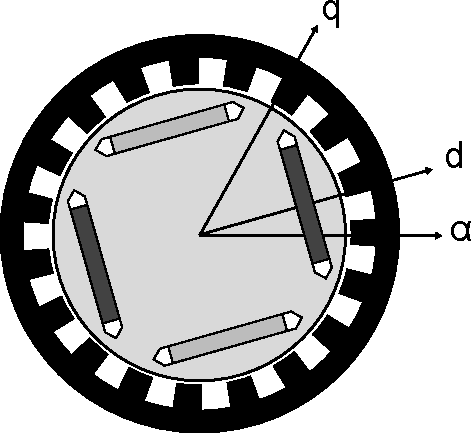
\includegraphics[width=0.5\columnwidth]{Slike/Inkscape/IPMSM.pdf}
    \caption{\label{IPMSM} Presek IPMSM stroja.}
\end{figure}


\section{Model IPMSM} \label{motor}

V pogonu se uporablja simetričen trofazni stroj, katerega matematično opišemo v RKS s sledečima enačbama:

\begin{equation} \label{motorModelD}
    u_d = R_si_d+L_d\frac{di_d}{dt}-\underbrace{\omega L_qi_q}_{e_d}
\end{equation}

\begin{equation} \label{motorModelQ}
    u_q = R_si_q+L_q\frac{di_q}{dt}+\underbrace{\omega L_di_d + \omega\Psi_{TM}}_{e_q}
\end{equation}

, kjer sta $e_d$ in $e_q$ inducirani napetosti vzdolžne in prečne komponente.
\\
Navor, ki ga tvori IPMSM pa je naslednji:

\begin{equation}
    M_{el} = \frac{3}{2}p\Bigl(\underbrace{\Psi_{TM}i_q}_{M_{sinhr}}+\underbrace{(L_d-L_q)i_qi_d}_{M_{rel}}\Bigr)
\end{equation}



\section{Brezsenzorsko vodenje FOC}

Pri vodenju FOC uporabljamo kaskadni regulator, kjer se notranja zanka uporablja za regulacijo toka, zunanja pa regulacijo hitrosti (ali pozicije). Za poenostavitev vodenja se uporablja Clarkina
transformacija s katero trofazne veličine predstavimo v dveh ortogonalnih oseh, $\alpha$ in $\beta$ v statorskem koordinatnem sistemu (SKS). Veličine v SKS pa transformiramo v RKS z uporabo Parkove
transformacije, te pa se uporabljajo za vodenje tokov v vzdolžni in prečni osi. Pri SPMSM se uporablja striktno prečna komponenta za tvorjenje navora, tok vzdolžne komponente pa se regulira na ničelni
tok. Pri IPMSM pa je poleg sinhronskega navora prisoten tudi reluktančni navor, katerega lahko izokristimo za doseganje višjega navora z metodo maksimalnega navora na Ampere (MTPA)
\cite{ambrovzivc2016elektrivcni}.

Za doseganje višje končne vrtilne hitrosti pa se uporablja metoda slabljenja polja, kjer se z vzdolžno komponento slabi magnetno polje rotorskih magnetov in s tem zniža efekt inducirane
napetosti\cite{ambrovzivc2016elektrivcni}.

Na sliki \ref{FOCshema} je prikazana shema FOC regulacije sistema, ki vključuje HFSI algoritem. Ker se v sistemu ne uporablja nobena od omenjenih metod, je željena vrednost toka vzdolžne komponente enaka 0.

\begin{figure}[!htbp]
    \centering
    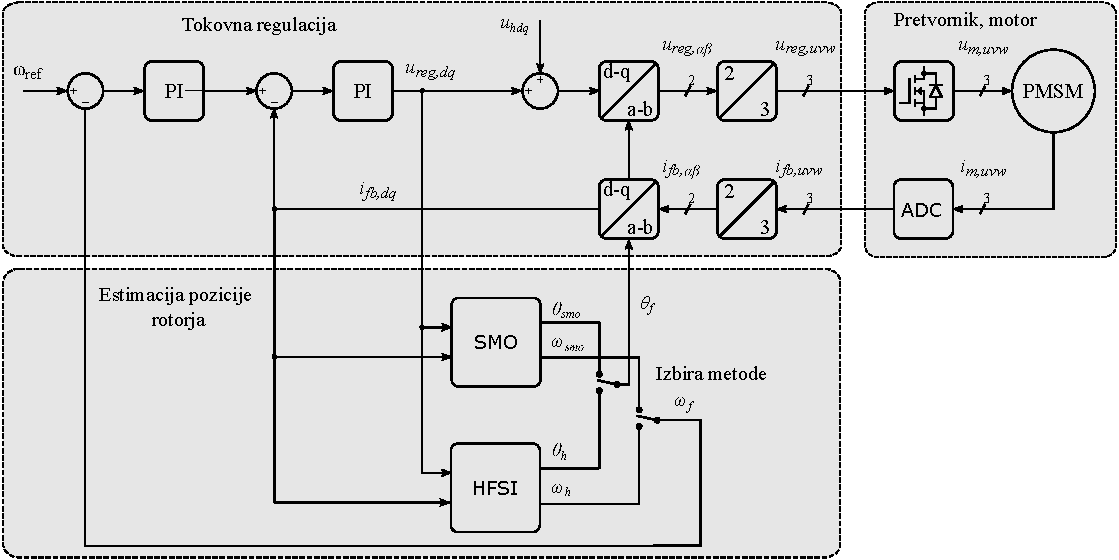
\includegraphics[width=0.75\columnwidth]{Slike/Inkscape/FOC-eps-converted-to.pdf}
    \caption{\label{FOCshema} Shema brezsenzorskega FOC vodenja.}
\end{figure}

Ker se uporablja brezsenzorsko vodenje, je potrebno odklon rotorja estimirati iz merjenega toka. Pri višji vrtilni hitrosti se za to uporablja metoda (TODO - SMO PLL ?). Ta z uporabo modela motorja, merjenega
kota in znane pritisnjene napetosti estimira inducirano napetost, ki pa je funkcija odklona rotorja. Z uporabo fazno zaklenjene zanke (PLL) pa se iz inducirane napetosti estimira odklon rotorja TODO
citat.
Opisana metoda odpove pri nižjih hotrostih, kjer je inducirana napetost premajhna oziroma ničelna v nevrtečem stanju. V takih pogojih se uporabljajo metode, ki izkoriščajo izraženost polov \cite{ThreeYearsOfExperience}. Skupnost
vseh takih metod je vzbujanje statorja z dodatno napetostno komponento, ki je superponirana osnovno, ki tvori navor. Nekatere metode vzbujajo stator med vsako PWM periodo, druge uporabljajo pulzirajoč
signal, ki vzbuja le vzdolžno komponentno in tako minimizira moteč navor zaradi vzbujalne napetosti. HFSI algoritem pa uporablja vrteč signal, ki vzbuja tudi prečno komponentno. 

Zaznavanje začetne pozicije rotorja v nevrtečem stanju je prav tako pomembna, saj omogoča takojšnje delovanje z visoko učinkovitostjo, prav tako pa izniči možnost vrtenja v napačno smer. Za zaznavanje
začetne pozicije se ponovno izkorišča izraženost polov in je opisano v \cite{IPDBoussak}.

\chapter{Delovanje HFSI} \label{teorija}

%TODO povsod odklon HKS od RKS uporabi določen simbol za ta kot

V tem poglavju je opisano delovanje HFSI metode. Ker metoda stoji na predpostavki, da se induktivnost v d in q smeri razlikujeta, je najprej predstavljena induktivnost stroja, nato je
opisan postopek vzbujanja statorja z visoko frekvenco, nato pa izračun estimiranega kota. Na koncu je opisana integracija algoritma v FOC.
\\
V klasičnem FOC vodenju 3 faznega stroja se fazne veličine z uporabo Clarkine transformacije pretvorijo v 2 fazni sistem, nato pa z uporabo Parkove transformacije v d-q k.s. Pri HFSI metodi pa se
uporablja dodaten d-q k.s., HKS, v katerem vzbujamo stator in tokovni odziv uporabljamo za vodenje odklona HKS. Na sliki \ref{koordinatniSistem} so prikazani uporabljeni k.s.

\begin{figure}[!htbp]
    \centering
    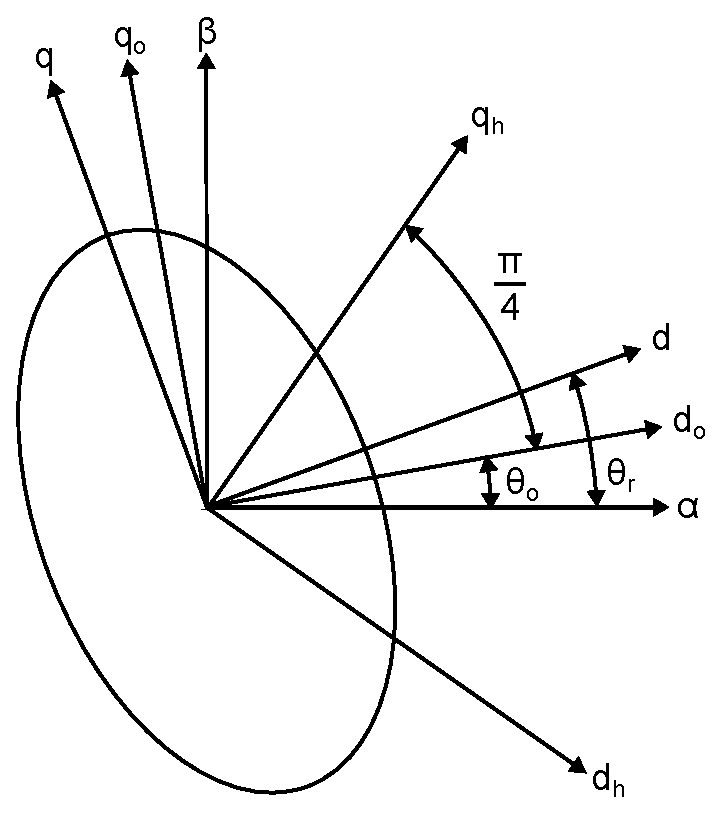
\includegraphics[width=0.75\columnwidth]{Slike/Inkscape/koordinatniSistem.eps}
    \caption{\label{koordinatniSistem} Koordinatni sistemi uporabljeni v HFSI algoritmu}
\end{figure}

\section{Induktivnost stroja}
Razlika induktivnosti v d in q osi RKS se pojavi zaradi neheterogene sestave rotorja in je maksimalna v smeri q in minimalna v smeri d. Kot je prikazano na sliki TODO, je
HKS zamaknjen za kot $\frac{pi}{4}$ od RKS. Ko je napaka estimacije kota enaka 0, sta induktivnosti v smeri d in q k.s. HKS enaki. Induktivnosti lahko matematično zapišemo kot:

\begin{center}
    $L_{dh} = L_p + L_r cos(2\Delta\theta + \frac{pi}{2})$

    $L_{qh} = L_p + L_r cos(2\Delta\theta - \frac{pi}{2})$
\end{center}

, kjer je $\Delta\Theta$ napaka estimirane pozicije.
\\
Zapis induktivnosti s kosinusoidno funkcijo je le poenostavitev realnosti, ker niso vsi stroji konstruirani tako, da potek sledi sinusoidni krivulji. Oblika induktivnosti namreč pride iz geometrije
rotorja - oblike izraženih polov rotorja. Dejanski potek induktivnosti je prikazan na sliki \ref{induktivnostStroja}, kjer je bila ta pomerjena z RLC metrom ene same faze, drugi dve pa sta bili
odklopljeni. Poleg tega nam odziv kvari tudi vzdolžni in prečni tok, kot bo prikazano v naslednjem poglavju.

\begin{figure}[!htbp]
    \centering
    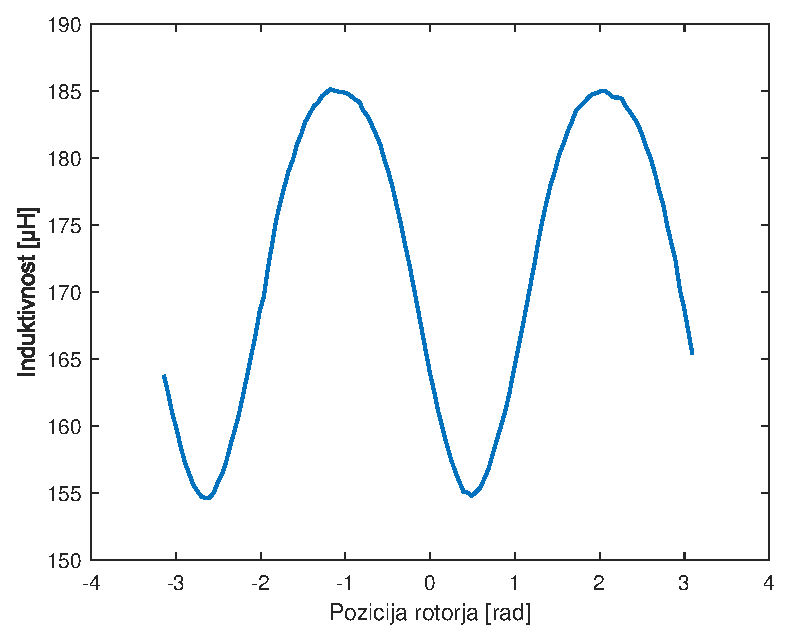
\includegraphics[width=1\columnwidth]{Slike/induktivnostStroja.eps}
    \caption{\label{induktivnostStroja} Induktivnost stroja}
\end{figure}

%To drži, dokler je d-q k.s. poravnan z rotorjem. Pri FOC
%vodenju je d-os vzporedna z magnetno osjo rotorja, q-os pa je ortogonalna na njo. HKS pa ni poravnan z rotorjem in tudi ne drži, da bo induktivnost v q smeri tega k.s. najvišja in v d smeri najmanjša.
%To je odvisno od naklona med HKS in RKS.
%Slika TODO prikazuje induktivnost v smeri d in q v odvisnosti od odklona HKS od RKS.

\section{Vzbujanje z visoko frekvenco v d-q prostoru}
Ker se bo pozicija estimirala preko induktivnosti, je le to potrebno meriti. En od načinov merjenja induktivnosti je preko merjenja impedance - tuljavo vzbujamo z izmenično napetostjo amplitude $U_s$
neke frekvence $f_s$ in iz pomerjenega toka izračunamo upornost. Ta je za tuljavo, ki ima upornost $R_L$ in induktivnost $L$ naslednja:

\begin{center}
    $Z_L = R_L + X_L = R_L + j2\pi f_sL$
\end{center}

Če je $R_L$ znatno manjši od $X_L$ lahko zapišemo:

\begin{center}
    $Z_L \cong j2\pi f_sL$
\end{center}

Skozi tuljavo z nekim vzbujanjem, bi tekel naslednji tok:

\begin{center}
    $I = \frac{U}{Z_L} = \frac{U_s \sin{(2\pi f_s)}}{2\pi f_sL}$
\end{center}

Amplituda tokovnega odziva, bi tako bila:

\begin{center}
    $\hat{I} = \frac{U_s}{2\pi f_sL}$
\end{center}

V enačbah \ref{motorModelD} in \ref{motorModelQ} ob predpostavitvi, da se rotor ne vrti oz vrti z nizko frekvenco, zanemarimo člen inducirane napetosti in motor poenostavimo v RL vezje:

\begin{equation} \label{motorModelD}
    u_d = R_si_d+L_d\frac{di_d}{dt}
\end{equation}

\begin{equation} \label{motorModelQ}
    u_q = R_si_q+L_q\frac{di_q}{dt}
\end{equation}

Pri dovolj visoki frekvenci vzbujanja se tudi predpostavi, da je statorska ohmska upornost mnogokrat manjša od reaktance in zapišemo amplitudo tokovnega odziva vzdolžne in prečne komponente HKS
odvisne od induktivnosti.

\begin{center}
    $\hat{I}_{dh} = \frac{U_s}{2\pi f_sL_{dh}}$
\end{center}

\begin{center}
    $\hat{I}_{qh} = \frac{U_s}{2\pi f_sL_{qh}}$
\end{center}

Ko vstavimo induktivnosti $L_{dh}$ in $L_{qh}$ v zgornjo enačbo, dobimo amplitudo tokovnega odziva v odvisnosti od odklona HKS od RKS.
\begin{center}
    $\hat{I}_{dh} = \frac{U_s}{2\pi f_s (L_p + L_r cos(2\Delta\theta + \frac{\pi}{2}))}$
\end{center}

\begin{center}
    $\hat{I}_{qh} = \frac{U_s}{2\pi f_s (L_p + L_r cos(2\Delta\theta - \frac{\pi}{2}))}$
\end{center}

V realnem sistemu iz merjenega toka dobimo visoko frekvenčni odziv, ne pa direktno amplitude. To moramo izračunati iz odziva s pomočjo Fourierove transformacije. V digitalnih sistemih se velikokrat
uporablja hitra Fourierova transformacija (FFT), ki pa je za ta primer prepotratna, saj potrebujemo amplitudo signala pri le eni frekvenci - zato uporabimo Goertzelov algoritem.

Kot induktivnost stroja, so tudi tokovni odzivi poenostavitev realnega sistema. Lahko pričakujemo najnižjo vrednost amplitude tokovnega odziva v vzdolžni smeri in najvišjo v prečni, vendar bo oblika
in s tem tudi odklon, kjer sta odziva enake amplitude malo zamaknjena od pričakovane. To je prikazano na slikah \ref{tokovniOdzivKot0} in \ref{tokovniOdzivKot45}, kjer je odklon rotorja kot med
rotorjem - gnanim ročno - in FKS (HKS je za pi/4 zamaknjen od FKS).

\begin{figure}[!htbp]
    \centering
    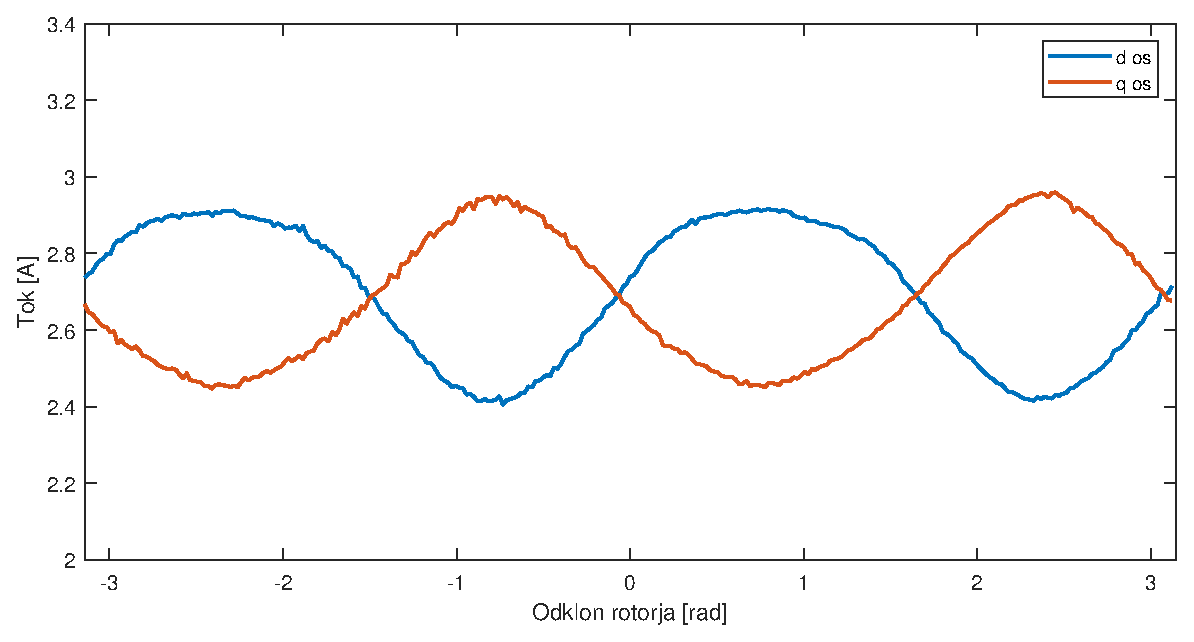
\includegraphics[width=1\columnwidth]{Slike/tokovniOdzivKot0.eps}
    \caption{\label{tokovniOdzivKot0} Primer vključitve slike.}
\end{figure}

\begin{figure}[!htbp]
    \centering
    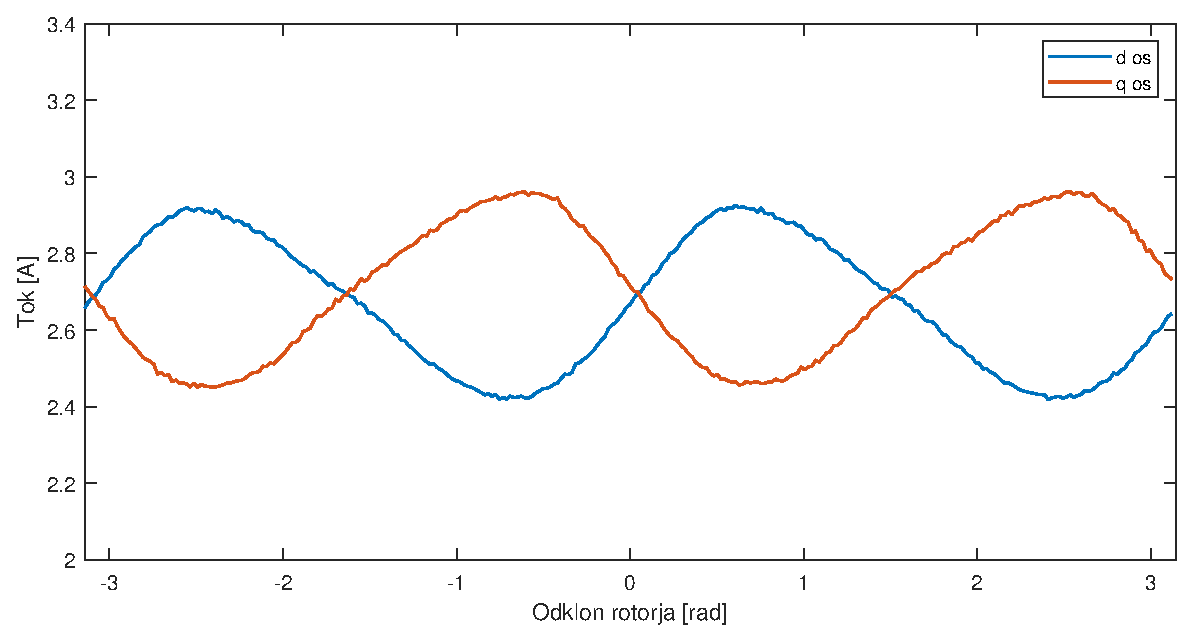
\includegraphics[width=1\columnwidth]{Slike/tokovniOdzivKot45.eps}
    \caption{\label{tokovniOdzivKot45} Primer vključitve slike.}
\end{figure}

Na sliki \ref{tokovniOdzivKot0} je bil koordinatni sistem HKS poravnan s SKS - torej je bila vzdolžna od HKS poravnana z osjo $\alpha$ SKS, na sliki \ref{tokovniOdzivKot45} pa je bil HKS za 45 stopinj
odmaknjen od SKS. Opazimo, da je že tukaj nekaj odstopanja. V delovanju HFSI metode, kjer se HKS vrti napram SKS, bomo dobili različne odzive, odvisno od trenutnega odklona HKS. 
\\
Dodatno nam odziv kvarita vzdolžna in prečna tokova, ki ju uporabljamo za tvorjenje navora, pri metodah MTPA in slabljenje polja pa poleg prečne tudi tok vzdolžne komponente ni ničelen. Ta dva tokova
dodatno magnetita jedro rotorja, kar spremeni magnetne razmere v stroju, kot je prikazano na slikah \ref{tokovniOdzivId} - \ref{tokovniOdzivIq_IqAmp}:

\begin{figure}[!htbp]
    \centering
    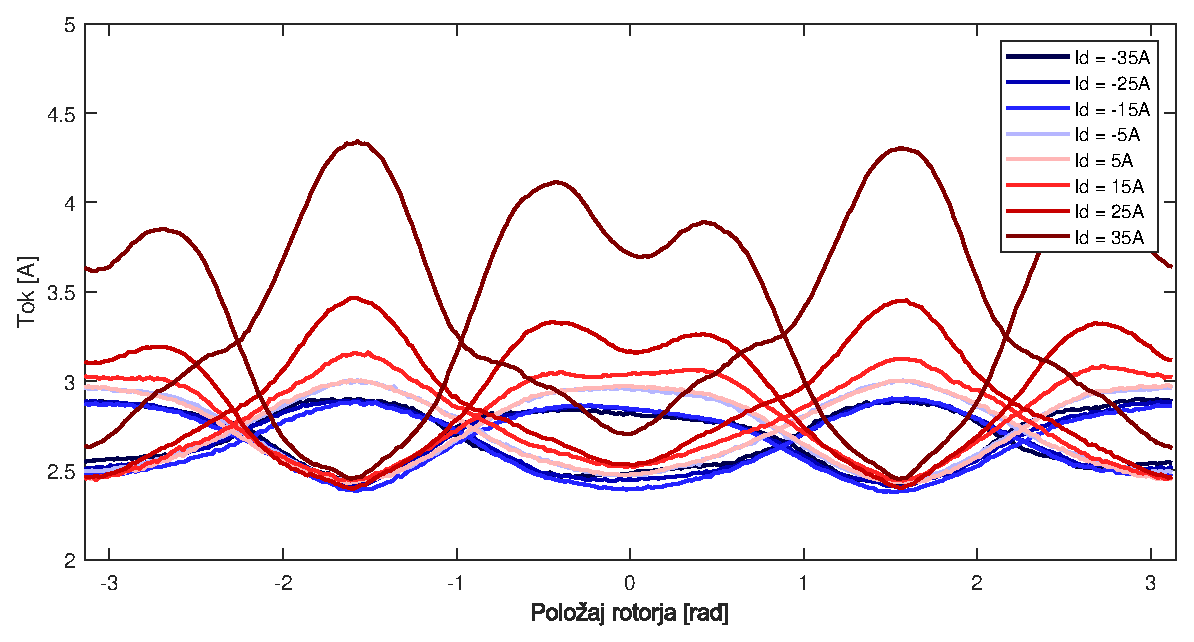
\includegraphics[width=1\columnwidth]{Slike/tokovniOdzivId.eps}
    \caption{\label{tokovniOdzivId} Primer vključitve slike.}
\end{figure}

Vidimo, da vzdolžni tok možno zmanjša induktivnost v d smeri, v q smeri pa je odziv relativno konstanten pri različnih vzdolžnih tokovnih.
Vzbujanje s prečnim tokom pa je prikazano na dveh slikah, na sliki \ref{tokovniOdzivIq_IdAmp} je prikazan odziv v vzdolžni smeri HKS, na sliki \ref{tokovniOdzivIq_IqAmp} pa prečni. 

\begin{figure}[!htbp]
    \centering
    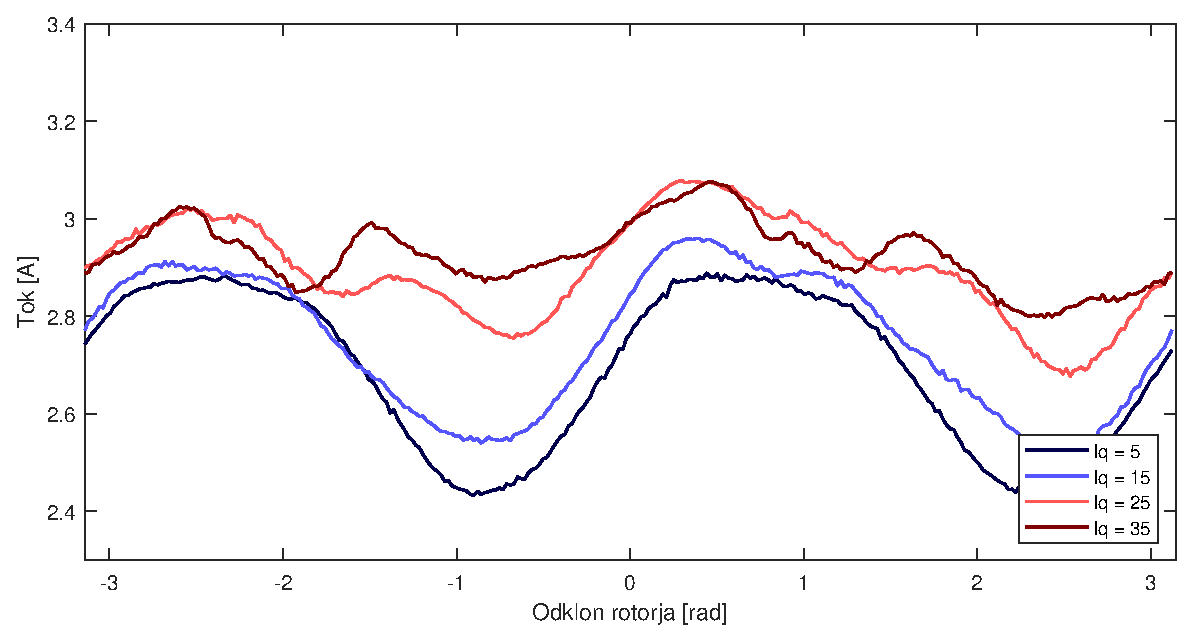
\includegraphics[width=1\columnwidth]{Slike/tokovniOdzivIq_IdAmp.eps}
    \caption{\label{tokovniOdzivIq_IdAmp} Primer vključitve slike.}
\end{figure}

\begin{figure}[!htbp]
    \centering
    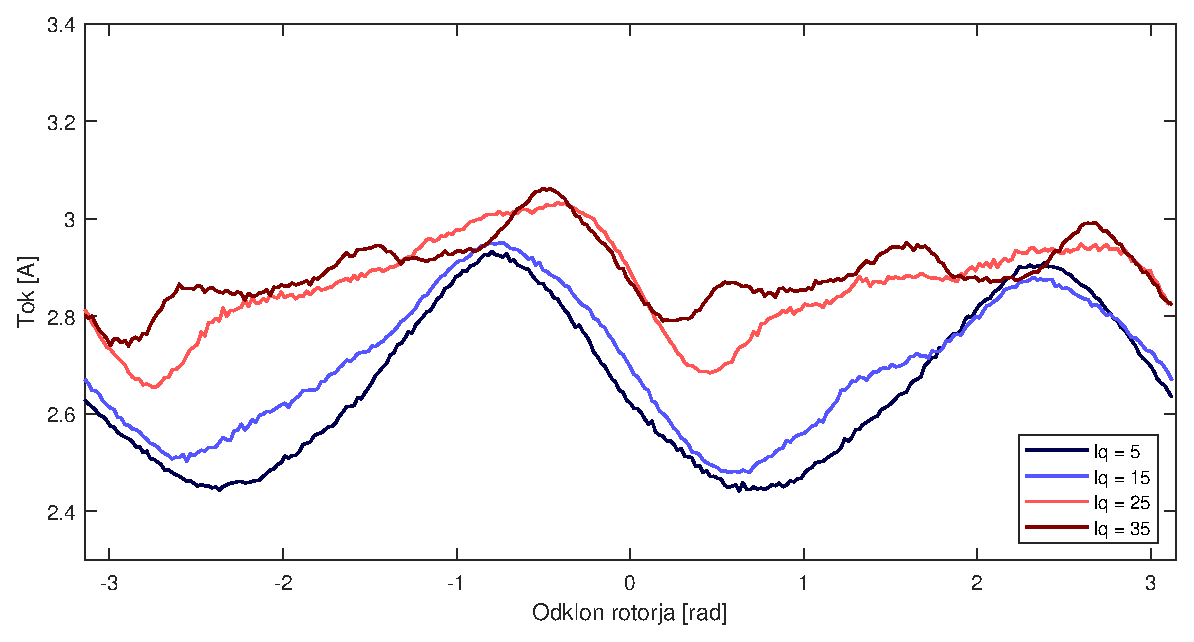
\includegraphics[width=1\columnwidth]{Slike/tokovniOdzivIq_IqAmp.eps}
    \caption{\label{tokovniOdzivIq_IqAmp} Primer vključitve slike.}
\end{figure}
 
Moramo pa se zavedati tudi dejstva, da pri brezsenzorskem vodenju ne poznamo prave pozicije rotora in imamo na voljo samo približno vrednost. Tudi v poenostavljenem vodenju kjer uporabljamo samo
prečni tok za tvorjenje navora, bomo v primeru napake estimirane pozicicje rotorja v RKS imeli nek neničelni vzdolžni tok. Slike \ref{tokovniOdzivId} - \ref{tokovniOdzivIq_IqAmp}, kjer je bila
pozicija rotorja znana z dajalnikom pozicije, prikazujejo samo odziv sistema v primeru ali vzdolžnega ali prečnega toka. V realnem sistemu pa se bo pozicija estimirala in bo imela neko napako. Zato si
poglejmo amplitude tokovnih odzivov v primeru, kjer ne poznamo pozicije rotorja. HKS je kot prej od FKS odmaknjen za $\frac{\pi}{4}$ in poravnan s SKS, vrednost prečnega toka je parametrizirana, vzdolžni tok se vodi na
ničelno vrednost, z vrtenjem rotorja pa umetno ustvarjamo napako estimirane pozicije.

\begin{figure}[!htbp]
    \centering
    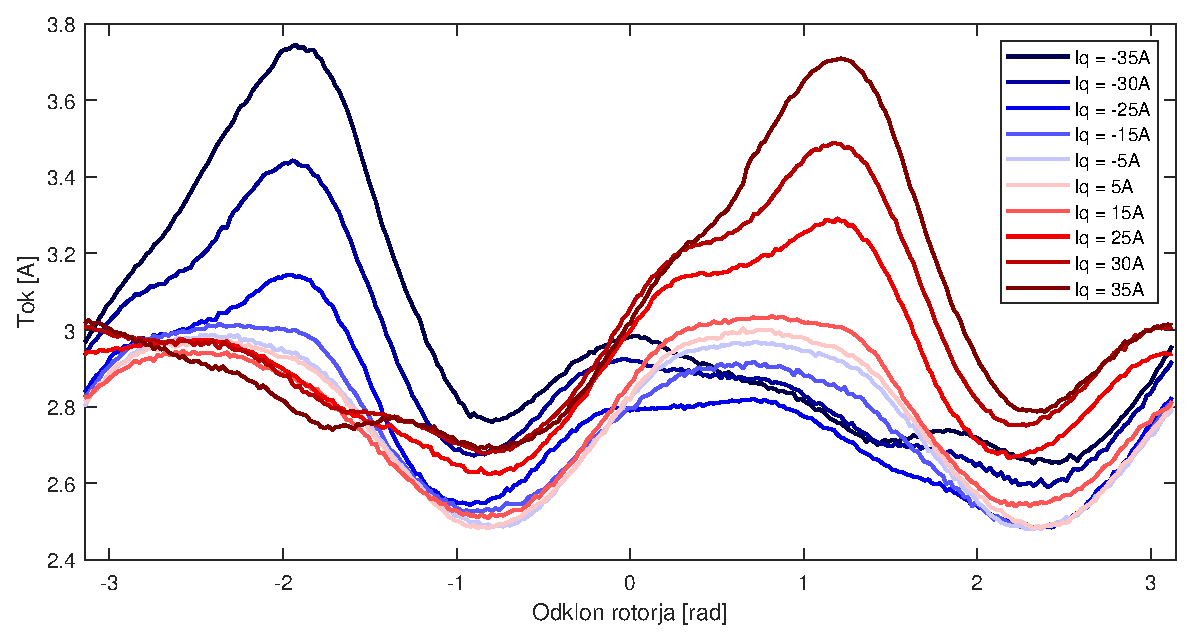
\includegraphics[width=1\columnwidth]{Slike/tokovniOdzivIs_IdAmp.eps}
    \caption{\label{tokovniOdzivIs_IdAmp} Primer vključitve slike.}
\end{figure}

\begin{figure}[!htbp]
    \centering
    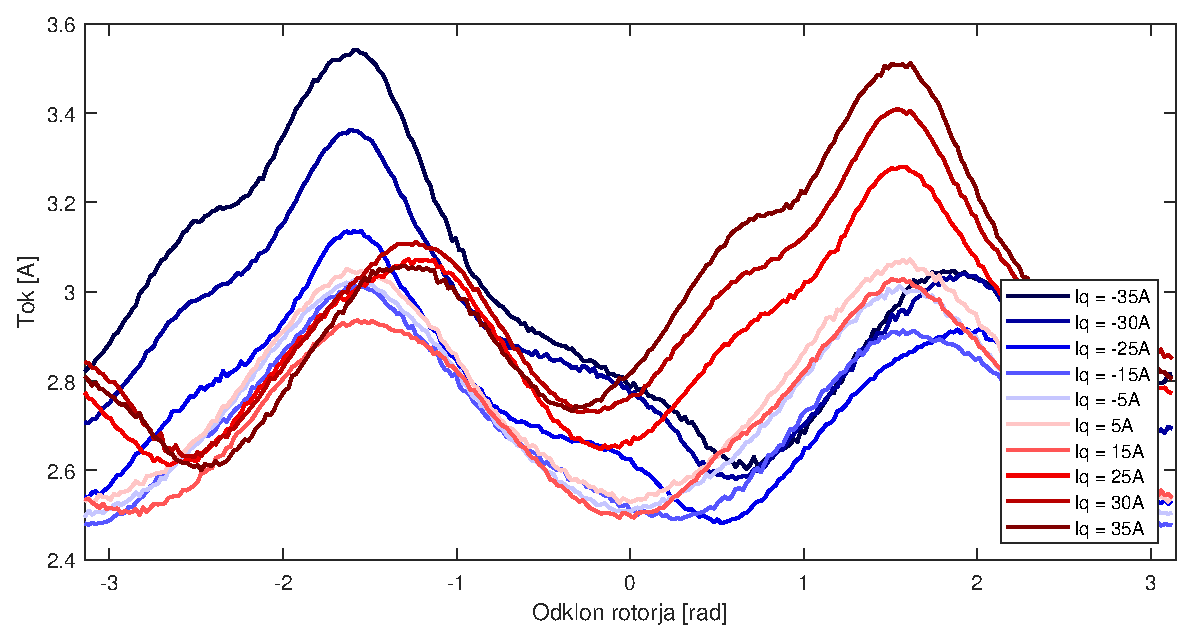
\includegraphics[width=1\columnwidth]{Slike/tokovniOdzivIs_IqAmp.eps}
    \caption{\label{tokovniOdzivIs_IqAmp} Primer vključitve slike.}
\end{figure}

%-> Odziv odvisen od odklona hfsi, verjetno zaradi magnetne asimetrije
%
%-> Odziv v odvnosti od Id
% 
%-> odizv v odvisnosti od Iq, oblika ni tok pomembna kt to da se ti regulirana veličina spreminja z Iq/Id. Predstavitev regulirane veličine v naslednjem poglavju 
%
%Odziva $\hat{I}_{dh}$ in $\hat{I}_{qh}$ sta enaka, ko je kot $\Delta\theta$ enak faktorju $\frac{pi}{2}$, kar je pomembno 


\section{Izračun pozicije rotorja}

Amplitudi tokovnega odziva v d smeri in q smeri HKS sedaj odštejemo in to razliko uporabimo kot regulirano veličino:

\begin{center}
    $\hat{I}_{e} = \hat{I}_{qh} - \hat{I}_{dh}$
\end{center}

V primeru, kjer sta vzdolžni in prečni tok enaka nič in vzbujamo stator le z visoko frekvenco v HKS, je $\hat{I}_{e}$ dokaj sinusoidne oblike, kot je vidno na sliki \ref{reguliranaVelicinaIdq0}.

\begin{figure}[!htbp]
    \centering
    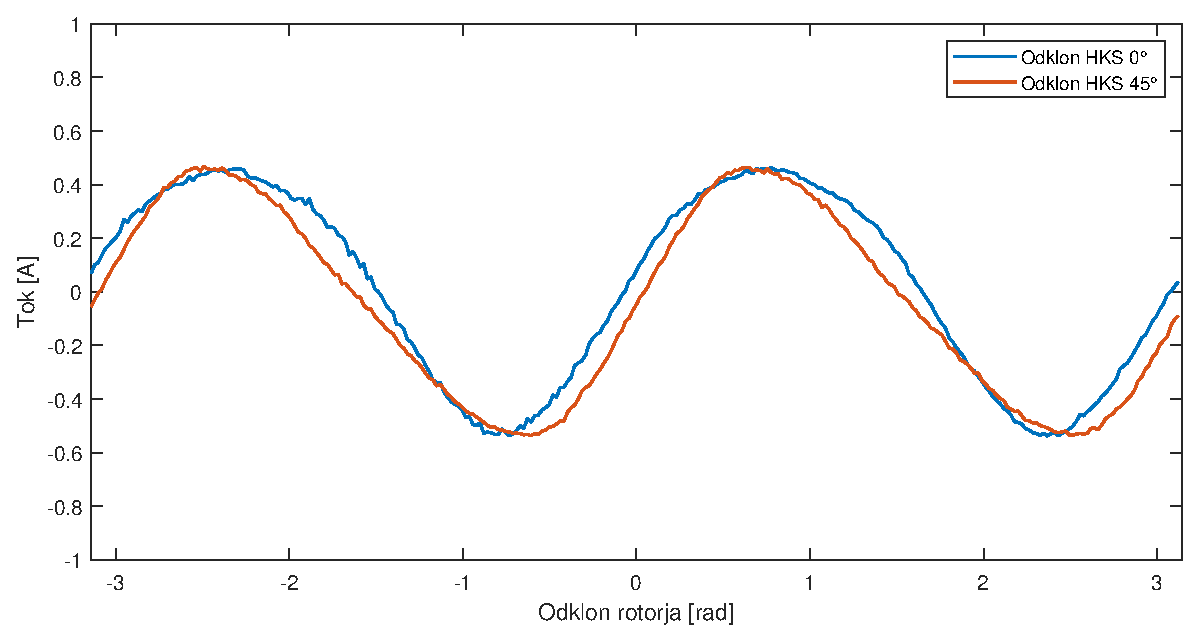
\includegraphics[width=1\columnwidth]{Slike/reguliranaVelicinaIdq0.eps}
    \caption{\label{reguliranaVelicinaIdq0} Primer vključitve slike.}
\end{figure}

Iz slike \ref{reguliranaVelicinaIdq0} je razvidno, da že samo odklon HKS od SKS vpliva na lokacijo ničelne napake. V prejšnjem poglavju je so bili prikazani odzivi v odvisnosti od prečnega in
vzdolžnega toka. $\hat{I}_{e}$ v teh pogojih je naslednja:

\begin{figure}[!htbp]
    \centering
    \includegraphics[width=1\columnwidth]{Slike/reguliranaVelicinaId.eps}
    \caption{\label{reguliranaVelicinaId} Primer vključitve slike.}
\end{figure}


Vzdolžni tok nam močno poveča amplitudo regulirane veličine $\hat{I}_{e}$, s tem pa se okoli delovne točke naklon regulirane veličine tudi močno poveča. To nam spremeni ojačanje povratne zanke in s
tem dinamiko sistema.

\begin{figure}[!htbp]
    \centering
    \includegraphics[width=01\columnwidth]{Slike/reguliranaVelicinaIq.eps}
    \caption{\label{reguliranaVelicinaIq} Primer vključitve slike.}
\end{figure}

Prečni tok pa nam amplitudo regulirane veličine zmanjša, opazi pa se tudi, da v dveh točkah ($\frac{\pi}{2}$ in $-\frac{\pi}{2}$) regulirana veličin ni več linearna. Pri višjih tokovih se celo izravna.
V teh točkah algoritem ni več stabilen, zato se mora izbrati prava delovna točka.
Opazimo pa, da kljub uporabi visokega prečnega toka pri ničtem odklonu ali odklonu za kot $\pi$ regulirana veličina ohranja naklon in delovna točka, kjer $\hat{I}_{e} = 0$ se ne spreminja.
\\
Da dobimo realnen pogled na delovanje algoritma v brezsenzorskem načinu, pa moramo pogledati, kakšen bo odziv toka $\hat{I}_{e}$ v odvisnosti od napake estimirane pozicije rotorja. Če na sliki
\ref{tokovniOdzivIs} odštejemo amplitudi odziva v prečni in vzdolžni komponenti dobimo vrednost toka $\hat{I}_{e}$ v odvisnosti od napake estimacije pozicije rotorja. To je prikazano na sliki
\ref{reguliranaVelicinaIs}:

\begin{figure}[!htbp]
    \centering
    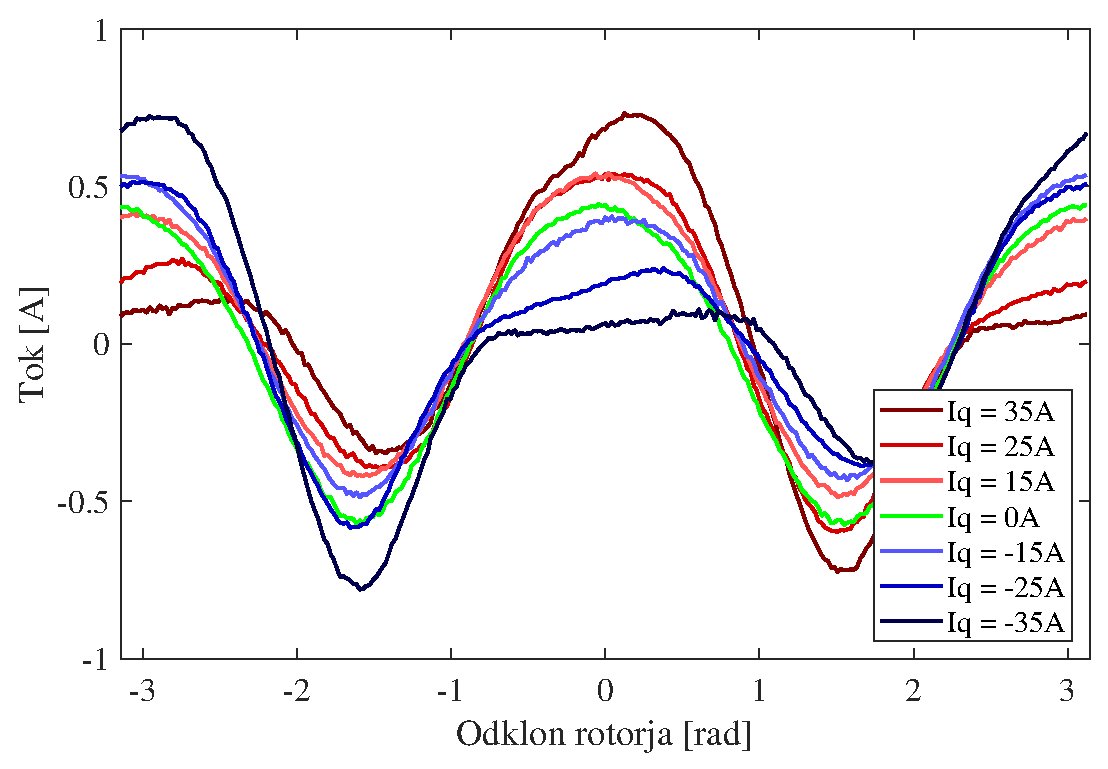
\includegraphics[width=1\columnwidth]{Slike/reguliranaVelicinaIs.eps}
    \caption{\label{reguliranaVelicinaIs} Primer vključitve slike.}
\end{figure}

Če poskrbimo, da bo imel tok $\hat{I}_{e}$ vedno ničelno vrednost, bo tako tudi HKS odklonjen od rotorskega koordinatnega sistema za $\frac{\pi}{4}$. Opazimo da se okoli delovne točka, ko je napaka
ocenjenega kota majhna, se $\hat{I}_{e}$ spremninja linearno. Od željene vrednosti regulirane veličina, torej nič, odštejemo dejansko vrednost $\hat{I}_{e}$ in to vstavimo v PI regulator. Izhod
regulatorja je regulirna veličina, to je veličina preko katere vplivamo na regulirano. V tem primeru je to vrtilna hitrost $\omega_o$, ki jo integriramo da dobimo pozicijo HKS, katero pa v povratni zanki
uporabimo za nov izračun $\hat{I}_{e}$. 

Tako z regulacijo $\hat{I}_{e}$ na nič dosežemo, da sta amplitudi tokovnega odziva v vzdolžni in prečni komponenti HKS enaki. Iz tega sledi, da je HKS od RKS odklonjen za $\frac{\pi}{4}$. Do pozicije
rotorja pridemo s preprostim izračunom:

\begin{equation}
    \theta_{r} = \theta_{h} - \frac{\pi}{4}
\end{equation}

\section{Vpliv mrtvega časa pretvornika}
Kaj je mrtvi čas, zakaj je potreben in kako vpliva na sistem. Realna napetost na statorju zaradi mrtvega časa, kako to vpliva na sistem etc. 
\\
V praktičnem sistemu, kjer se uporablja močnostni pretvornik imamo opravka s preklopi visokih in nizkih tranzistorjev. Ko je odprt nizek fet, je fazna napetost 0V, ko je odprt visok fet pa je fazna
napetost enaka napajalni. Med preklopom iz 0V in 24V pa je za kratek čas potrebno izklopiti oba, saj v primeru, kjer prevajata oba nastane nizko-impedančna pot, ki povzroči kratek stik. Čas, ko sta
izklopljena oba se imenuje mrtvi čas in povzroča napetostno napako \cite{ambrovzivc2016elektrivcni}. Ta napaka je odvisna od 

Za delovanje HFSI algoritma pa poleg osnovne harmonske komponente za tvorjenje navora vzbujamo stator še z visoko frekvenčno komponento. V primeru, kjer stator vzbujamo samo z visoko frekvenco, bi
mrtvi čas vedno vplival na odziv in njegov vpliv bi bil konstanten. Ko pa vzbujamo še s konstantnim prečnim ali vzdolžnim tokom, pa vidimo vpliv mrtvega časa samo, ko osnovna harmonska tokovna komponenta
zamenja polariteto. To lahko potrdimo z meritvami na realnem sistemu, kjer HKS odmaknemo od RKS za $\frac{\pi}{4}$ in v FKS vzbujamo stator s konstantnim tokom, rotor pa počasi vrtimo. Pričakovali bi
konstantno in enako amplitudo VF tokovnega odziva v prečni in vzdolžni komponenti HKS, vendar na sliki \ref{mrtviCas} opazimo, da je na šestih pozicijah odziv popačen in da je magnituda napake dokaj linearno odvisna
od mrtvega časa. Modra barva označuje amplitudo VF odziva prečne komponente, rdeča pa vzdolžne. Temnejši kot so odzivi, večji je mrtvi čas. 

\begin{figure}[!htbp]
    \centering
    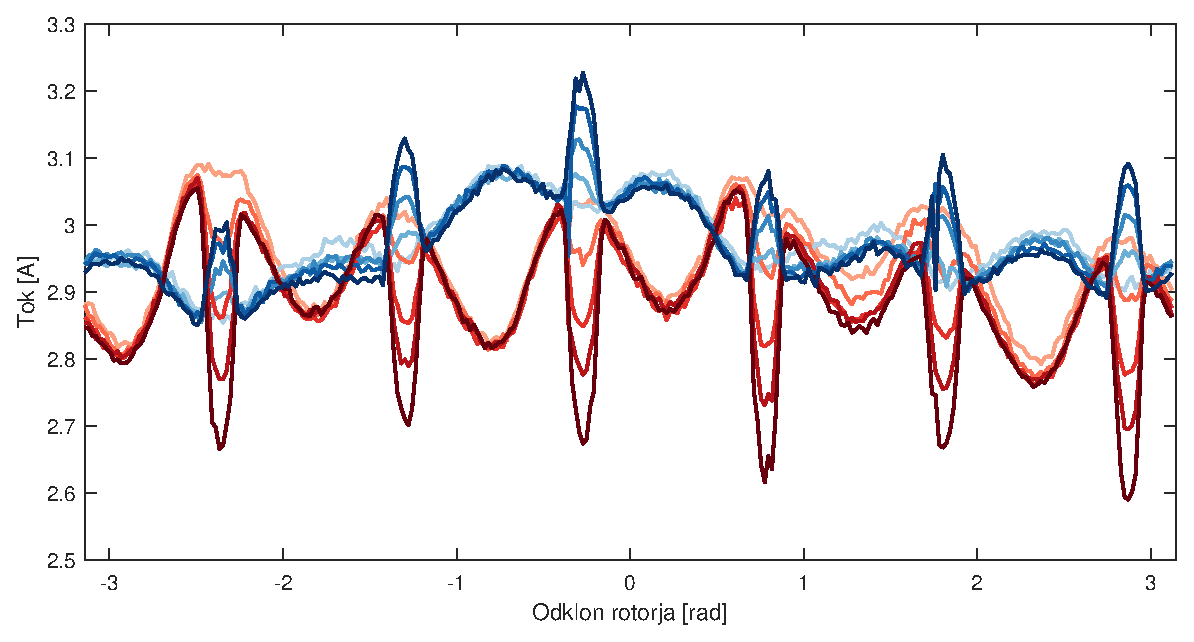
\includegraphics[width=1\columnwidth]{Slike/mrtviCas.eps}
    \caption{\label{mrtviCas} Odvisnost popačenja amplitude odziva od dolžine mrtvega časa}
\end{figure}

Prav tako lahko potrdimo, da je mrtvi čas odvisen od napajalne napetosti, prikazano na sliki \ref{mrtviCasNapetost}. Odziv je bil pomerjen pri napetostih 16V, 24V in 32V, kjer je temnejša barva večja
napetost.


\begin{figure}[!htbp]
    \centering
    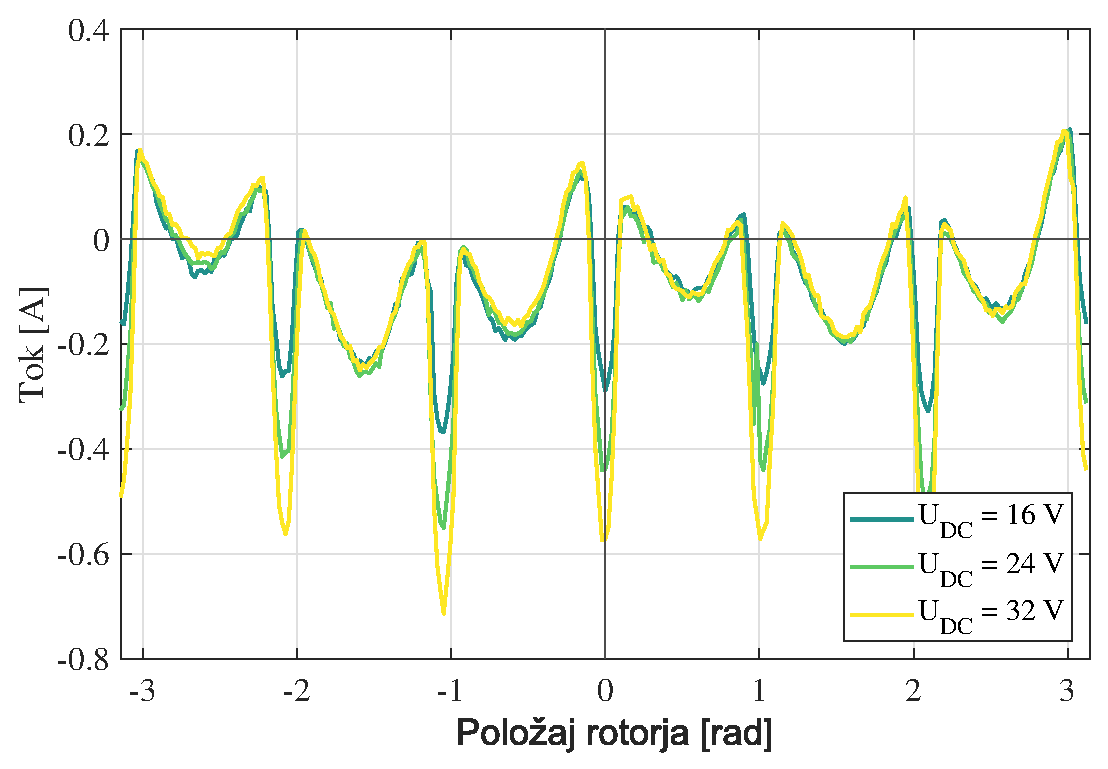
\includegraphics[width=1\columnwidth]{Slike/mrtviCasNapetost.eps}
    \caption{\label{mrtviCasNapetost} Odvisnost popačenja amplitude odziva od napajalne napetosti }
\end{figure}

Dodatno lahko pokažemo, da se vpliv mrtvega časa začne kazati takrat, ko začne VF tokovni odziv menjati polariteto. // TODO dodaj graf in pokomentiraj

Takšno popačenje amplitude odziva naravno vpliva na oceno pozicije, saj bo PI regulator poiskušal zmanjšati napako in to tako, da bo spremenil odklon HKS na mesto, kjer imata odziva enako vrednost.
Vpliv mrtvega časa na oceno pozicije pa je prikazan v zadnjem poglavju.

\chapter{Integracija v FOC} \label{integracija}

Za uspešno implementacijo HFSI algoritma, ga je potrebno tudi pravilno integrirati v celotno FOC vodenje. Potrebno je poskrbeti za pravilno inicializacijo algoritma, filtriranje tokovne povratne
zanke, zadnji element pa je preklop v delovanje SMO načina, ko vrtilna hitrost doseže dovolj visoko vrednost.

\section{Inicializacija HFSI}

Ker s HFSI algoritmom nismo zmožni ocenjevati polaritete rotorja, potrebujemo za pravilno smer vrtenja poskrbeti, da je začetna pozicija znana. Pred zagonom HFSI zaznamo začetno pozicijo rotorja, ki
se začne uporabljati že od samega začetka delovanja HFSI. Ker je HKS od RKS odklonjen za $\frac{\pi}{4}$, je začetna vrednost kota HKS enaka ocenjeni začetni vrednosti RKS z odklonom $\frac{\pi}{4}$.
\\
Pri delovanju HFSI tokovna povratna zanka vključuje tudi VF komponento, ki jo je potrebno izfiltrirati. Uporabimo zaporni pasovni filter (BSF). Filtriranja ne smemo izvesti v SKS, saj je tam VF
komponenta različne frekvence, ki je odvisna tudi od vrtilne hitrosti HKS. Zato filtriramo v RKS, kjer ima konstantno frekvenco in sicer tako, s katero vzbujamo stator v HKS. Ker filtriramo v RKS, pa
lahko filtrirane tokove $I_d$ in $I_q$ direktno uporabimo za tokovno regulacijo. 
\\
Ob zagonu prvih nekaj period vzbujalnega signala FOC regulatorje izklopimo, da se prehodni pojav pasovnih filtrov ustali. 

\section{Začetni kot in izbira minimuma}

\section{Preklop v SMO}

Proti koncu delovanja HFSI algoritma, ko je vrtilna hitrost že dovolj visoka, da ocenjujemo pozicijo rotorja z inducirano napetostjo, je potrebno izvesti brezudarni preklop. Takoj po preklopu želimo,
da SMO začne delovati v pravilni delovni točki. To lahko dosežemo tako, da SMO deluje vzporedno s HFSI algoritmom. Ob preklopu tako samo izklopimo vzbujanje statorja. Ta način pa terja dodatne
kalkulacije, ki so lahko v določenih sistemih, kjer je nadvsem pomembna nizka cena in zato uporaba manj zmogljivih procesorjev, previsoke. Zato se uporabi drug način, ki pa ob preklopu postavi SMO v
željeno delovno točko. To pomeni, da je potrebno vsa notranja stanja postaviti na pravilno začetno vrednost. To vključuje notranja stanja modela, ki se uporablja za estimacijo inducirane napetosti,
ocenjeno hitrost in pozicijo PLL. Problem pri tej metodi pa je, da se je težko izogniti manjšim prenihajem, saj bo vedno prisotna napaka estimacije pozicije in hitrosti algoritma HFSI in ima zato SMO ob
preklopu že neko majhno napako. 

% TODO slika brezudarnega preklopa

\chapter{Eksperimenti}  \label{eksperimenti}

V tem poglavju je najprej opisano krmiljenje napetostnega pretvornika in merjenje toka, saj tudi to vpliva na algoritem. Na koncu so prikazane meritve realnega sistema, ki so bile zajete z
osciloskopom, interne spremenljivke, uporabljene v samem algoritmu, pa so bile v realnem času poslane na računalnik preko komunikacijskega protokola UART. 

TODO opis sistema ker proc driver etc?

\section{Trifazni PWM in meritev toka}

V sistemu se uporablja asimetričen PWM s fazno zamaknjenimi fazami. Največja prednost tega je preprosta implementacija krmiljenja napetosti in merjenje toka, slaba lastnost pa je večje valovanje
frekvence PWM-ja. Potek faznih napetosti je prikazan na sliki \ref{PWM}, kjer se vidi fazni zamak faz - fazno sta zamaknjeni prva in druga faza za merjenje toka. $t_{PWM}$ je perioda PWM, $t_{MEAS}$
pa je časovni zamik poteka faze za tokovno meritev. $t_0$ do $t_5$ pa so časi, kjer faze spremenijo polariteto. Ti časi določajo, kakšna je efektivna napetost na fazah in se izračunajo kot je
prikazano z enačbo \ref{izracunPWM}. $t_0$, $t_1$ in $t_2$ se ne spreminjajo, saj takrat merimo tok, $t_3$, $t_4$ in $t_5$ pa so odvisni od željenih faznih napetosti. Implementacija na mikrokrmilniku
potrebuje še dodatno pretvorbo iz časa v število taktov PWM periferije krmilnika.

\begin{equation} \label{izracunPWM}
\begin{gathered}
    t_0 = 0  \\
    t_1 = t_{MEAS}  \\
    t_2 = 2t_{MEAS}  \\
    t_3 = t_{MID} + u_uV_c  \\
    t_4 = t_{MID} + t_{MEAS} + u_vV_c \\
    t_5 = t_{MID} + 2t_{MEAS} + u_wV_c
\end{gathered}
\end{equation}

$t_{MID}$ ni polovica $t_{PWM}$, saj smo rezervirali $2t_{MEAS}$ periode za meritev toka. Zato je $t_{MID}$ enak polovici $t_{MID} - 2t_{MEAS}$. $V_c$ pa je faktor za pretvorbo željenje napetosti v
čas in je preprosto razmerje med dolžino periode in napetostno zalogo. Napetostna zaloga - oziroma napajalna napetost - se aktivno meri, saj želimo da je dejanska napetost na izhodu enaka željeni. Pri
FOC vodenju to praviloma ni problem, saj tokovni regulatorji tok regulirajo. HFSI algoritem pa vsebuje tudi visokofrekvenčno napetostno vzbujanje in se predpostavlja, da je taka tudi na izhodu in ni
odvisna od napajalne napetosti. Če bi ta bila odvisna, bi pri višjih napajalnih napetostih dobili večji tokovni odziv, kar pa si lahko predstavljamo kot ojačanje povratne zanke - to pa bi sledilo v
spremembo dinamike regulacijskega sistema, ki ga HFSI vsebuje.

\begin{figure}[!htbp]
    \centering
    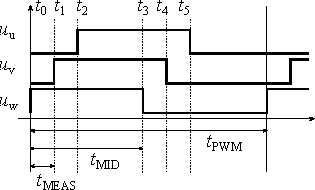
\includegraphics[width=1\columnwidth]{Slike/Inkscape/PWM.pdf}
    \caption{\label{PWM} Pulzno širinska modulacija močnostnega pretvornika }
\end{figure}

// TODO dodaj sliko pwmjev in shunt meritve


%V sistemu se uporablja asimetričen PWM in je prikazan na sliki TODO. Največja prednost tega je preprosta implementacija krmiljenja napetosti in merjenje toka, slaba lastnost pa je večje valovanje
%frekvence PWM-ja. Pretvorba željene napetosti FOC vodenja v preklope tranzistorjev napetostnega pretvornika se stori z modulacijo prostorskih vektorjev (SVM). Željena napetost se na strani pretvornika
%vidi kot časovno zaporedje nekaj prostorskih vektorjev (odvisno od napetosti). Ti so lahko ali ničelni vektor - (0,0,0) ali (1,1,1) - ali pa aktivni vektor. Aktivni vektorji so stanja, kjer ima vsaj
%ena izmed medfaznih napetosti neničelno vrednost. Povprečna napetost na vsaki izmed faz v eni periodi PWM je tako enaka željeni vrednosti FOC vodenja. 
%
%Napetost faze iz ničelnih vektorjev izračunamo kot povprečje napetosti ene periode:
%
%
%
%
%\\
%Na začetku sekvence prostorskih vektorjev se za merjenje toka uporabljata dva aktivna vektorja, nato pa z uporabo dve ničelnih in dveh aktivnih vektorjev sestavimo željeno izhodno napetost. 
%
%Asimetričen PWM ima na začetku zaporedja dva aktivna vektorja, ki se uporabljata za merjenje toka, nato sledi ničelni vektor, nato pa ponovno dva aktivna vektorja in nakoncu ničelni vektor. To
%zaporedje predstavlja ničelno napetost, kar je tudi razvidno iz povprečnih vrednosti faz. Vse ostale kombinacije faznih napetosti pa se sestavijo 

%\section{Merjenje toka} 
%Ključna lastnost asimetričnega PWM je, da se prva dva vektorja po časovni dolžini ne spreminjata. Tako nam ni potrebno spreminjati točke, kjer se meri tok. 
%TODO operacijc v driverju?


\section{Rezultati} \label{rezultati}

Vpliv izbire napačnega začetnega minimuma

Vpliv mrtvega časa na oceno kota

Vpliv Iq na oceno kota

PID tuning

Razlika odziva pri nizkem/srednjem navoru in visokem/vsiljena pozicija

\subsection{Primerjava ...} \label{graf1}

Podsekcije za različne meritve, primerjave, odvisnosti veličin, potrjevanje teoretične osnove iz prejšnega poglavja, itd...

%******************************* ZAKLJUČEK *************************************
\chapter{Zaključek} \label{zakljucek}


%******************************* LITERATURA ************************************
\cleardoublepage\phantomsection\addcontentsline{toc}{chapter}{Literatura} % vnos literature v kazalo

% 1. način: BibTeX
\bibliographystyle{ieeetrslo}
\bibliography{literatura}

% 2. način: neposreden vnos \begin{thebibliography}{99} \bibitem{vir1} C. Su, H. Ke in T. Hubing, ``Overview of Electromagnetic Modeling Software'' [Online], v \textit{25th Annual Review of Progress
%    in Applied Computational Electromagnetics, March 8 - March 12, 2009 - Monterey, California}. Monterey, 2009, str. 736-741. Dosegljivo: \url{http://www.clemson.edu/ces/cvel/pdf/ACES09-736.pdf}.
%    [Dostopano: 23.8.2017]. \bibitem{vir2} T. Hubing et al., ``Survey of Current Computational Electromagnetics Techniques and Software'' [Online]. \textit{Clemson University Vehicular Electronics
%    Laboratory (CVEL)}: Clemson, ZDA, CVEL-08-011.2, 21.9.2008. Dosegljivo: \url{http://www.clemson.edu/ces/cvel/Reports/CVEL-08-011.2.pdf}. [Dostopano: 23.8.2017]. \bibitem{vir3} \textit{The
%    Electromagnetic Radiation Spectrum Poster} [Online]. Dosegljivo: \url{http://www.unihedron.com/projects/spectrum/}. [Dostopano: 23.8.2017]. \end{thebibliography}

%******************************* DODATEK ***************************************
\appendix

\end{document}
%%%%%%%%%%%%%%%%%%%%%%%%%%%%%%%%%%%%%%%%%%%%%%%%%%%%%%%%%%%%%%%%%%%%%%%%%%%%%%%%%%%%%%%%%%%%%%%%%%%%%%%%%%%%%%%%%%%%%%%%
